\documentclass{cheat-sheet}

\pdfinfo{
  /Title (Zusammenfassung Markovketten)
  /Author (Tim Baumann)
}

\usepackage{bbm} % Für 1 mit Doppelstrich (Indikatorfunktion)
\usepackage{mathtools} % psmallmatrix environment
\usepackage{nicefrac}

\usepackage{tikz}
\usetikzlibrary{matrix}

% Kleinere Klammern
\delimiterfactor=701

% TODO: Include-File für Stochastik

\newcommand{\Alg}{\mathfrak{A}} % (Mengen-)Algebra
\renewcommand{\P}{\mathbb{P}} % Wahrscheinlichkeitsmaß
\newcommand{\E}{\mathbb{E}} % Erwartungswert
\newcommand{\ind}{\mathbbm{1}} % Indikatorfunktion
\newcommand{\iid}{i.\,i.\,d.} % identisch unabhängig verteilt
\DeclareMathOperator{\ggT}{ggT} % größter gemeinsamer Teiler

\DeclareMathOperator{\var}{Var} % Varianz
\DeclareMathOperator{\cov}{Cov} % Kovarianz
\DeclareMathOperator{\cor}{Cor} % Korrelation

\definecolor{DefinitionColor}{rgb}{0.7,0.2,0.0}
\newcommand{\Defn}[1]{\textcolor{DefinitionColor}{#1}}

\begin{document}

\raggedcolumns % stretche Inhalt nicht über die gesamte Spaltenhöhe

\maketitle{Zusammenfassung Markovketten}

% Vorlesung vom 4.5.2017

% Kapitel II. Abzählbare Markovketten
\section{Abzählbare Markovketten}

% §2.1. Rekurrenz und Transienz

\begin{nota}
  Sei im Folgenden $\{ Z_n \}$ eine Markovkette auf einem abzählbaren Zustandsraum~$E$.
\end{nota}

% 2.1
\begin{defn}
  Für $x \in E$ und $n \in \N$ definiere die ZV \Defn{$\tau_x^{(n)}$} induktiv durch
  \[ \begin{array}{r c l}
    \tau_x^{(1)} &\coloneqq& \inf\,\Set{n > 0}{Z_n = x} \in \N \cup \{ \infty \} \\
    \tau_x^{(k)} &\coloneqq& \inf\,\Set{n > \tau_x^{(k-1)}}{Z_n = x}, \enspace k > 1.
  \end{array} \]
  (Beachte: $\tau_x^{(k)}$ ist eine messbare Abbildung.)
\end{defn}

\begin{bem}
  Ferner gilt $\{ \tau_x^{(k)} = n \} \in \sigma(Z_0, Z_1, \ldots, Z_n)$.
\end{bem}

\begin{defn}
  Für $x, y \in E$ sei
  $\Defn{F(x, y)} \coloneqq P(\tau_y^{(1)} < \infty \mid Z_0 = x)$
\end{defn}

% 2.2
\begin{lem}
  Für alle $x, y \in E$ und $k \geq 1$ gilt
  \[ P(\tau_y^{(k)} < \infty \mid Z_0 = x) = F(x, y) \cdot F(y, y)^{k-1}. \]
\end{lem}

\begin{bem}
  Setze $\Defn{\widetilde{\ell}(y)} \coloneqq {\sum}_{k=j}^\infty \ind \{ Z_k = y \}$.
  Dann gilt
  \[ P(\tau_y^{(k)} < \infty \mid Z_0 = x) = P(\widetilde{\ell} \geq k \mid Z_0 = x). \]
\end{bem}

% 2.3
\begin{defn}
  Ein Zustand $x \in E$ heißt
  \begin{itemize}
    \item \emph{absorbierend}, falls $p(x, x) = 1$,
    \item \emph{rekurrent}, falls $F(x, x) = 1$ und
    \item \emph{transient}, falls $F(x, x) < 1$.
  \end{itemize}
\end{defn}

\begin{bem}
  Absorbierende Zustände sind rekurrent.
\end{bem}

% ausgelassenes  Beispiel: a+1 Zustände nebeneinander, der linke und rechte sind absorbierend, die dazwischen haben eine Übergangswahrscheinlichkeit von 1/2 nach links und 1/2 nach rechts

% ausgelassenes Beispiel: Irrfahrt auf \N
% Falls $p \leq \nicefrac{1}{2}$, so ist Anfangszustand rekurrent
% Falls $p > \nicefrac{1}{2}$, so ist Anfangszustand transient
% Parondo-Paradoxon

\begin{bsp}
  In der Markovkette
  \begin{center}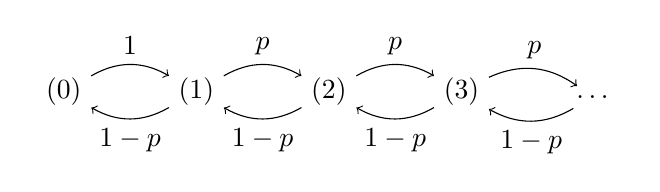
\begin{tikzpicture}
    \matrix [matrix of nodes, column sep=1cm, row sep=0.8cm] {
      \node (N0) {(0)}; &
      \node (N1) {(1)}; &
      \node (N2) {(2)}; &
      \node (N3) {(3)}; &
      \node (N4) {\ldots}; \\
    };
    \draw[->, bend left=30] (N0) to node [above] {$1$} (N1);
    \draw[->, bend left=30] (N1) to node [below] {$1 - p$} (N0);
    \draw[->, bend left=30] (N1) to node [above] {$p$} (N2);
    \draw[->, bend left=30] (N2) to node [below] {$1 - p$} (N1);
    \draw[->, bend left=30] (N2) to node [above] {$p$} (N3);
    \draw[->, bend left=30] (N3) to node [below] {$1 - p$} (N2);
    \draw[->, bend left=30] (N3) to node [above] {$p$} (N4);
    \draw[->, bend left=30] (N4) to node [below] {$1 - p$} (N3);
  \end{tikzpicture}\end{center}
  ist (0) genau dann rekurrent, falls $p \leq \nicefrac{1}{2}$, ansonsten transient.
  \TODO{genauer!}
\end{bsp}

% 2.6
\begin{defn}
  Die \emph{Anzahl der Besuche} in~$y \in E$ ist
  \[
    \Defn{\ell(y)} \coloneqq {\sum}_{k=0}^\infty \ind \{ Z_k = y \}.
  \]
  Die \emph{Green'sche Funktion} von $\{ Z_n \}$ ist $G : E \times E \to \cinterval{0}{\infty}$ mit
  \[
    \Defn{G(x, y)} \coloneqq \E(\ell(y) \mid Z_0 = x).
  \]
\end{defn}

\begin{bem}
  $
    \begin{array}[t]{r c l}
      G(x, y) &=& \E \left( {\sum}_{k=0}^\infty \ind \{ Z_k = y \} \mid Z_0 = x \right) \\
      &=& {\sum}_{k=0}^\infty P(Z_k = y \mid Z_0 = x) \\
      &=& \delta_{xy} + {\sum}_{k=1}^\infty p^{(k)}(x, y).
    \end{array}
  $
\end{bem}

% 2.7
\begin{satz}
  Für alle $x, y \in E$ gilt
  \[
    G(x, y) = 
    \begin{cases}
      F(x, y)/(1 - F(y, y)) & \text{falls $x \neq y$}, \\
      1/(1 - F(y, y)) & \text{falls $x = y$}. \\
    \end{cases}
  \]
\end{satz}

\begin{kor}
  $x$ ist rekurrent $\iff$ $G(x, x) = \infty$
\end{kor}

% 2.8
\begin{satz}
  Ist $x \in E$ rekurrent und $F(x, y) > 0$, so ist $y$ auch rekurrent und $F(x, y) = F(y, x) = 1$.
\end{satz}

\iffalse
% 2.9
\begin{interp}
  %Die Aussage kann man wie folgt deuten:
  $F(x, y) > 0$ bedeutet, dass nach jedem Besuch in~$x$ der Zustand $y$ auch besucht wird mit positiver Wahrscheinlichkeit und die Rekurrenz von~$x$ bedeutet, dass $x$ unendlich oft besucht wird.
  Der Satz sagt, dass dann auch $y$ unendlich oft besucht wird.
\end{interp}
\fi

% 2.9
\begin{bem}
  $F(x, y) > 0 \iff \ex{n \geq 1} p^{(n)}(x, y) > 0$
\end{bem}

% 2.10
\begin{defn}
  $\{ Z_n \}$ heißt \emph{irreduzibel}, falls $\fa{x, y \in E} F(x, y) > 0$.
\end{defn}

% 2.11
\begin{satz}
  Sei $\{ Z_n \}$ irreduzibel.
  Dann sind entweder alle Zustände rekurrent oder alle Zustände transient.
\end{satz}

% Vorlesung vom 9.5.2017

% 2.12
\begin{satz}
  Irreduzible Ketten auf endlichen Räumen sind rekurrent.
\end{satz}

% §2. Rekurrenz und Transienz von Irrfahrten
\section{Rekurrenz und Transienz von Irrfahrten}

\begin{situation}
  $\{ Z_n \}$ ist eine Irrfahrt auf $\Z^d$, \dh{}
  \[ p(x, y) = p(0, y - x) =: q(y - x). \]
  Mit and. Worten: Die \textit{Zuwächse} $\{ Z_n - Z_{n-1} \}_{n \geq 1}$ sind \iid{} ZVn.
\end{situation}

\begin{bsp}
  Einfache Irrfahrt auf~$\Z$: \quad
  $p(0, 1) = p$, $p(0, -1) = q = 1 - p$
\end{bsp}

%Für welche Werte von $p$ ist diese Irrfahrt rekurrent/transient?

In diesem Fall kann man die Greensche Funktion exakt berechnen:

\[
  \begin{array}{r c l}
    G(x, x) &=& G(0,0) \\
    &=& {\sum}_{m=0}^\infty p^{(m)}(0, 0) \\
    &=& 1 + {\sum}_{n=1}^\infty p^{(2n)}(0, 0) \\
    &=& 1 + {\sum}_{n=1}^\infty \tbinom{2n}{n} p^n (1-p)^n \\
    &=& 1 + {\sum}_{n=1}^\infty \tbinom{2n}{n} 4^{-n} (4 p (1-p))^n \\
    &=& (1 - 4 p (1-p))^{-1/2} \\
    &=& 1/\abs{2p - 1}
  \end{array}
\]

% 2.13
\begin{satz}
  Sei $\{ Z_n \}$ eine Irrfahrt auf~$\Z$ mit
  \[ \E \abs{Z_1 - Z_0} = {\sum}_{x \in \Z} \abs{x} p(0, x) < \infty. \]
  Dann gilt: \quad
  $
    \{ Z_n \} \text{ ist rekurrent} \iff {\sum}_{x \in \Z} \, x p(0, x) = 0.
  $
\end{satz}

\begin{defn}
  Die \emph{einfache symmetrische Irrfahrt auf $\Z^d$} ist die translationsinvariante Markovkette mit
  \[
    p(0, \pm e_i) = \tfrac{1}{2 d} \quad \text{für } i = 1, \ldots, d.
  \]
\end{defn}

\begin{bem}
  Für einfache symmetrische Irrfahrten gilt:
  \[
    p^{(2n)}(x, x) = \qquad \sum_{\mathclap{\substack{k_1, \ldots, k_d \in \N \\ k_1 + \ldots + k_d = n}}} \qquad \frac{(2n)!}{(k_1!)^2 \cdots (k_d!)^2} (\frac{1}{2d})^{2n}
  \]

  Für $d = 2$ gilt $p^{(2n)}(0, 0) = \left[ \tbinom{2n}{n} (\tfrac{1}{2})^{2n} \right]^2$.
  Mit der Stirling'schen Formel folgt $p^{(2n)}(0, 0) \approx \tfrac{1}{\pi n}$.
  Somit gilt $\sum p^{(2n)}(0,0) = \infty$.
\end{bem}

\begin{fazit}
  Die zweidimensionale einfache symm. Irrfahrt ist rekurrent.
\end{fazit}

% Vorlesung vom 11.5.2017

\begin{bem}
  Man kann zeigen:
  Für einfache symm. Irrfahrten auf~$\Z^d$ gilt
  \[ p^{(2n)}(0,0) \leq C_d / n^{\nicefrac{d}{2}} \]
  für eine Konstante $C_d > 0$.
  Somit ist die einfache Irrfahrt transient für alle $d \geq 3$.
\end{bem}

\begin{defn}
  $\Defn{\varphi(t)} \coloneqq {\sum}_{x \in \Z^d} e^{i (t \cdot x)} p(0, x)$ \quad
  für $t \in \R^d$
\end{defn}

\begin{bem}
  Da die Zuwächse $\{ Z_n - Z_{n-1} \}$ \iid{} sind, gilt
  \[ {\sum}_{x \in \Z^d} \, e^{i (t \cdot x)} p^{(n)}(0, x) = \varphi^n(t), \quad n \geq 1 \]

  \textit{Inversionsformel}: \quad
  $p^{(n)}(0, x) = \tfrac{1}{(2 \pi)^d} \Int{\cointerval{-\pi}{\pi}^d}{}{e^{- i (t \cdot x)} \varphi^n(t)}{t}$
\end{bem}

\begin{satz}
  Für jede Irrfahrt $\{ Z_n \}$ auf $\Z^d$ gilt
  \[ G(0, 0) = \left( \frac{1}{2 \pi} \right)^d \lim_{\lambda \uparrow 1} \Int{t \in \cointerval{-\pi}{\pi}^d}{}{Re(\tfrac{1}{1 - \lambda \varphi(t)})}{t} = \infty \]
\end{satz}

\begin{bsp}
  Für die einfache symm. Irrfahrt $\{ Z_n \}$ auf~$\Z^d$ ist
  \[
    \varphi(t) = \tfrac{1}{d} {\sum}_{k=1}^d \cos(t_k)
  \]
  Mit der Ungleichung $1 - \cos(u) \geq c_0 u^2$ für alle $u \in \cinterval{- \pi}{\pi}$ folgt
  \[
    \varphi(t) \geq \tfrac{c_0}{d} \abs{t}^2.
  \]
  Es folgt
  \[
    \tfrac{1}{1 - \lambda \varphi(t)} \leq \tfrac{d}{\lambda c_0} \abs{t}^{-2}
  \]
  Die Funktion $\abs{t}^{-2}$ ist auf $\cointerval{-\pi}{\pi}^d$ für jedes $d \geq 3$ integrierbar.
  Somit ist die einfache Irrfahrt auf $\Z^d$, $d \geq 3$, transient.
\end{bsp}

% 2.16
\begin{satz}
  Jede irreduzible Irrfahrt auf $\Z^d$ mit $d \geq 3$ ist transient.
\end{satz}

% 2.17
\begin{bsp}
  Sei $\{ Z_n \}$ eine Irrfahrt auf $\Z$ mit $p(0, x) = p(0, -x)$.
  Gelte
  \[ x^\alpha p(0, x) \xrightarrow{x \to \infty} c \in \ointerval{0}{\infty} \]
  für ein $\alpha > 1$.
  Dann ist
  \[
    1 - \varphi(t) = \sum_{\mathclap{n=-\infty}}^\infty (1{-}\cos(nt)) p(0, n)
    \enspace \text{und} \enspace
    \frac{1 {-} \varphi(t)}{\abs{t}^{\alpha - 1}} = \sum_{\mathclap{n=-\infty}}^\infty \abs{n}^\alpha p(0, n) \abs{t} f(n t)
  \]
  mit $f(x) = (1 - \cos(x))/\abs{x}^\alpha$.
  Außerdem $\abs{n}^\alpha p(0, n) = c + \epsilon_n$, wobei $\epsilon_n \to 0$ für $\abs{n} \to \infty$.
  Es folgt
  \[
    \tfrac{1 - \varphi(t)}{\abs{t}^{\alpha - 1}} = \sum_{n=-\infty}^\infty c \abs{t} f(n t) + \sum_{n=-\infty}^\infty \epsilon_n \abs{t} f(n t).
  \]
  Für $t \to 0$ hat man
  \[
    \sum_{n=-\infty}^\infty \abs{t} f(n t) \to \Int{-\infty}{\infty}{f(x)}{x}
    \enspace \text{und} \enspace
    \sum_{n=-\infty}^\infty \epsilon_n \abs{t} f(n t) \to 0.
  \]
  Es folgt für $\alpha < 3$:
  \[ \lim_{t \to 0} \tfrac{1 - \varphi(t)}{\abs{t}^{\alpha - 1}} = c \Int{-\infty}{\infty}{\tfrac{1 - \cos(x)}{\abs{x}^\alpha}}{x} < \infty \]
  Folglich ist $\tfrac{1}{1 - \varphi(t)}$ für $\alpha < 2$ integrierbar und somit $\{ Z_n \}$ transient.

  Für $\alpha = 2$ ist $1/(1 - \varphi(t))$ in der Umgebung von null nicht integrierbar und damit $\{ Z_n \}$ rekurrent.

  Für $\alpha > 2$ ist $\sum \abs{x} p(0, x) < \infty$ und somit ist die Irrfahrt rekurrent, da der Erwartungswert der Zuwächse null ist.
\end{bsp}

% Vorlesung vom 16. Mai 2017

% §3. Erneuerungstheorie
\section{Erneuerungstheorie}

\begin{situation}
  Seien $\{ X_k \}_{k \geq 1}$ unabhängige ZVn mit Werten in~$\N$ und $P(X_k \geq 1) > 0$, wobei $\{ X_k \}_{k \geq 2}$ identisch vert. sind.
  Dann definiert
  \[
  Z_n \coloneqq {\sum}_{k=1}^n X_k + Z_0
  \]
  eine Irrfahrt $\{ Z_n \}_{n \geq 0}$ mit nicht-negativen Zuwächsen auf~$\Z$.
\end{situation}

\begin{ziel}
  Untersuche das asympt. Verhalten von $G(0, x)$.
\end{ziel}

\begin{defn}
  Die \emph{erzeugende Funktion} einer Folge $\{ a_n \}$ ist
  \[ A(s) \coloneqq \sum_{n=0}^\infty a_n s^n. \]
\end{defn}

% 2.18
\begin{bsp}
  Setze $p_k \coloneqq P(X_2 = k)$, $k \geq 0$.
  Wir nehmen an, dass
  \[ a \coloneqq \E[X_2] = {\sum}_{k=1}^\infty k p_k \in \ointerval{0}{\infty}. \]
  Definiere
  $q_k \coloneqq \tfrac{1}{a} {\sum}_{j=k}^\infty p_j$
  für $k \geq 1$.
  Dann ist ${\sum}_{k=1}^\infty q_k = 1$. \\
  Sei $X_1$ eine ZV mit $P(X_1=k) = q_k$, $k \geq 1$.
  Setze
  \[
    \begin{array}{r c l}
      f(s) &\coloneqq& {\sum}_{k=1}^\infty p_k s^k = \E[s^{X_2}], \enspace \abs{s} \leq 1 \\[0.1cm]
      g(s) &\coloneqq& {\sum}_{k=1}^\infty q_k s^k = \E[s^{X_1}] \\[0.1cm]
      \psi(s) &\coloneqq& {\sum}_{x=1}^\infty G(0, x) s^x, \enspace \abs{s} < 1
    \end{array}
  \]
  Dann gilt für $\abs{s} < 1$:
  \[ \psi(s) = {\sum}_{k=1}^\infty g(s) f(s)^{k-1} = g(s)/(1 - f(s)) \]
  Außerdem gilt:
  \[ g(s) = \tfrac{s}{a (1-s)} (1 - f(s)) \]
  Es folgt:
  \[ \psi(s) = \sum_{x=1}^\infty \tfrac{1}{a} s^x \]
  Somit ist $G(0, x) = \tfrac{1}{a}$.
\end{bsp}

% 2.19
\begin{satz}
  Angenommen, $\ggT \Set{k}{p_k > 0} = 1$.
  Dann gilt für jede Verteilung von~$X_1$, dass
  \[ G(0, x) \xrightarrow{x \to \infty} \tfrac{1}{a}. \]
\end{satz}

% 2.20
\begin{lem}
  Sei $g(\theta)$ integrierbar auf $\cointerval{-\pi}{\pi}$.
  Dann gilt
  \[
    \Int{\cointerval{-\pi}{\pi}}{}{e^{i \theta x} g(\theta)}{\theta} \xrightarrow{\abs{x} \to \infty}
    \quad (x \in \Z)
  \]
\end{lem}

% 2.21
\begin{lem}
  \begin{minipage}[t]{0.8 \linewidth}
    Seien alle $X_k$ identisch verteilt und $\ggT \Set{p}{p_k > 0} = 1$.
    Dann existiert $L \coloneqq {\lim}_{x \to \infty} G(0, x)$.
  \end{minipage}
\end{lem}

% 2.22
\begin{defn}
  Seien $\{ X_k \}_{k \geq 1}$ unabhängige, nichtneg. ZVn und seien $\{ X_k \}_{k \geq 2}$ identisch verteilt.
  Setze $Z_n \coloneqq {\sum}_{k=1}^n X_k$.
  Dann heißt
  \[
    \begin{array}{r c l l}
      \Defn{\eta(t)} &\coloneqq& \min\,\Set{k \geq 1}{Z_k > t} &
      \text{\emph{Erneuerungsprozess} und} \\
      \Defn{H(t)} &\coloneqq& \E[\eta(t)]
      & \text{\emph{Erneuerungsfunktion}.}
    \end{array}
  \]
\end{defn}

Falls $X_k$ nur Werte aus~$\N$ annimmt, so können wir das Verhalten von $H(t) - H(t-1)$ wie folgt beschreiben:
\[\begin{array}{r l}
  & H(t) = \E[\eta(t)] = \sum_{k=0}^\infty P(\eta(t) > k) = \sum_{k=0}^\infty P(Z_k \leq t) \\
  \rightsquigarrow & H(t) - H(t-1) = \sum_{k=0}^\infty P(Z_k = t) \xrightarrow{t \to \infty} 1/\E[X_2].
\end{array}\]

\begin{defn}
  $
    \begin{array}[t]{r c l l}
    \Defn{\gamma(t)} &\coloneqq& t - Z_{\eta(t)-1} \geq 0 & \text{heißt \emph{Overshoot},} \\
    \Defn{\chi(t)} &\coloneqq& Z_{\eta(t)} - t > 0 & \text{heißt \emph{Undershoot}.}
    \end{array}
  $
\end{defn}

\begin{satz}
  Sind die Bedingungen des letzten Satzes erfüllt, so gilt
  \[
    P(\gamma(t)=i, \chi(t)=j) \xrightarrow{t \to \infty} \frac{p_{i+j}}{\E[X_2]}
    \qquad \text{für alle } i \geq 0, j \geq 1.
  \]
\end{satz}

\begin{kor}
  $
    \begin{array}[t]{r c l}
      P(\gamma(t) = i) &\xrightarrow{t \to \infty}& \tfrac{1}{a} {\sum}_{k=i+1}^\infty p_k, \\[0.15cm]
      P(\gamma(t) = j) &\xrightarrow{t \to \infty}& \tfrac{1}{a} {\sum}_{k=j}^\infty p_k
    \end{array}
  $
\end{kor}

\TODO{Eine der Gleichungen im Korollar sollte $\chi$ beinhalten.}

% Vorlesung vom 23.5.2017

% §4. Positive Rekurrenz
\section{Positive Rekurrenz}

% 2.25
\begin{defn}
  $x \in E$ heißt \emph{positiv rekurrent}, falls $\E [\tau_x^{(1)} | Z_0=x] < \infty$
\end{defn}

\begin{bem}
  positive Rekurrenz $\implies$ Rekurrenz
\end{bem}

\begin{defn}
  Falls $x$ rekurrent, aber nicht positiv rekurrent ist, so heißt $x$ \emph{nullrekurrent}.
\end{defn}

% 2.26
\begin{lem}
  \begin{minipage}[t]{0.8 \linewidth}
    Sei $x$ ein positiv rekurrenter Zustand. \\
    Ist $F(x, y) > 0$ so ist auch~$y$ positiv rekurrent.
  \end{minipage}
\end{lem}

% 2.27
\begin{kor}
  Ist $\{ Z_n \}$ irreduzibel und $x_0 \in E$ positiv rekurrent, so gilt:
  \begin{itemize}
    \item alle Zustände sind positiv rekurrent
    \item $\Defn{m(x, y)} \coloneqq \E[ \tau^{(1)}_y | Z_0 = x ] < \infty$ für alle $x, y \in E$
  \end{itemize}
\end{kor}

% 2.28
\begin{defn}
  Die Zahl
  $d_x \coloneqq \ggT \Set{n \geq 1}{p^{(n)}(x,x) > 0}$
  heißt \emph{Periode} von~$x$.
  Falls $d = d_x$ für alle $x \in E$, so heißt $d$ \textit{Periode} der Kette~$\{ Z_n \}$.
\end{defn}

% 2.29
\begin{lem}
  Ist $\{ Z_n \}$ irreduzibel, so gilt $d_x = d_y$ für alle $x, y \in E$.
\end{lem}

% 2.30
\begin{satz}
  Es gibt eine Familie $\{ \pi_y \in \R_{> 0} \}_{y \in E}$, sodass
  \[ \fa{x, y \in E} p^{(n)}(x, y) \xrightarrow{n \to \infty} \pi_y \]
  genau dann, wenn
  \begin{itemize}
    \item $\{ Z_n \}$ irreduzibel und
    \item aperiodisch (\dh{} $d = 1$) ist und 
    \item ein $x_0$ existiert, sodass $m(x_0, x_0) < \infty$.
  \end{itemize}
  Die Folge $\{ \pi_y \}_{y \in E}$ ist die eindeutige Lösung zu
  \[
    \left\{
      \begin{array}{l}
        \sum_{y \in E} \abs{P_y} < \infty \\
        \sum_{y \in E} \pi_y = 1 \\
        \sum_{x \in E} \pi_x p(x, y) = \pi_y \text{ für alle } y \in E
      \end{array}
    \right.
  \]
  Es gilt $\pi_y = 1/m(y,y)$.
\end{satz}

% Vorlesung vom 30.5.2017

% 2.31
\begin{defn}
  Eine Verteilung $\{ \mu_x \}_{x \in E}$ auf~$E$ heißt \emph{stationär}, falls
  \[
    \mu_x = \sum_{y \in E} \mu_y p(y, x)
    \quad \text{für alle $x \in E$}
    \qquad \text{(kurz: $\mu = \mu P$).}
  \]
\end{defn}

\begin{bem}
  Für eine stationäre Verteilung $\{ \mu_x \}_{x \in E}$ gilt
  \[
    \mu_x = \sum_{y \in E} \mu_y p^{(n)}(y, x)
    \quad \text{für alle $x \in E$ und $n \in \N$}
  \]
\end{bem}

% 2.33
\begin{lem}
  Sei $x$ ein positiv rekurrenter Zustand.
  Dann definiert
  \[
    \Defn{\mu_y^{(x)}} \coloneqq \E[ \sum_{k=0}^{\tau_x^{(1)} - 1} \ind \{ Z_k = y | Z_0 = x \} ] / m(x, x)
  \]
  für alle $y \in E$ eine stationäre Verteilung $\{ \mu_y^{(x)} \}_{y \in E}$.
\end{lem}

% 2.34
\begin{satz}
  Sei $\{ Z_n \}$ eine irreduzible Kette.
  Dann gilt:
  \[
    \{ Z_n \} \text{ ist pos. rekurrent} \iff
    \{ Z_n \} \text{ hat eine stationäre Verteilung.}
  \]
  In diesem Fall ist die stationäre Verteilung eindeutig.
\end{satz}

% $\Defn{\sigma_x^n} \coloneqq \sup \Set{k \leq n}{Z_k = x} \in \{ - \infty, 0, \ldots, n \}$

% 2.35
\begin{satz}
  Eine irreduzible Kette auf einem endlichen Zustandsraum ist immer positiv rekurrent.
  Ferner existieren $C > 0$ und $q \in \ointerval{0}{1}$ mit
  \[
    P(\tau_y^{(1)} > n | Z_0 = x) < C q^n
    \quad \text{für alle $n \geq 1$ und $x, y \in E$.}
  \]
\end{satz}

% 2.36
\begin{satz}
  Sei $\{ Z_n \}$ irreduzibel und positiv rekurrent.
  Sei $f : E \to \R$ integrierbar bezüglich der stationären Verteilung $\{ \pi_x \}$, \dh{} $\sum_{x \in E} \abs{f(x)} \pi_x < \infty$.
  Dann gilt
  \[
    \tfrac{1}{n} \sum_{k=0}^{n-1} f(Z_k) \xrightarrow{\text{f.\,s.}} \sum_{x \in E} f(x) \pi_x
  \]
\end{satz}

\begin{bsp}
  Für $f(y) \coloneqq \ind \{ y = x_0 \}$ für eine $x_0 \in E$ erhalten wir
  \[ \tfrac{1}{n} \sum_{k=0}^{n-1} \ind \{ Z_k = x_0 \} \xrightarrow{\text{f.\,s.}} \pi_{x_0}. \]
  Es folgt mit majorisierter Konvergenz:
  \[ \tfrac{1}{n} \sum_{k=0}^{n-1} p^{(k)}(x, x_0) \xrightarrow{n \to \infty} \pi_{x_0}. \]
\end{bsp}

\begin{bsp}
  Sei $\{ Z_n \}$ irreduzibel, periodisch mit Periode $p > 1$.
  Dann gilt
  $p^{(dk)}(x_0, x_0) \xrightarrow d / m(x_0, x_0)$.
\end{bsp}

% 2.37
\begin{lem}
  Sei $\{ Z_n \}$ eine irreduzible Kette mit der Periode $d \geq 1$. \\
  Für jedes $x \in E$ existiert ein $m_x \geq 1$ mit
  \[
    p^{(md)}(x, x) > 0
    \text{für alle $m \geq m_x$.}
  \]
\end{lem}

\end{document}